% Originally: content/week-02.tex, \section{Compactness} (Corsin Week 2, Friday)

\section{Compactness}
\label{sec:compactness}

% Transition: Claude Opus 5 (High)
Compactness is the least self-explanatory definition in this chapter, so it is worth saying in
advance what it is \emph{for}. Finite sets are easy to handle: one can take a maximum, choose a
smallest radius, check finitely many cases. Infinite sets are not. Compactness is the property
that lets an infinite space be treated as if it were finite --- not because it is small, but
because every attempt to spread it out over infinitely many open pieces collapses back to
finitely many. \Cref{sec:why_compactness_matters} collects the three payoffs
(continuous images, attained extrema, uniform continuity); the definition below is what buys
them.

\begin{definition}[Compact metric space]
\label{def:compact_metric_space}
A metric space $(X,d)$ is \newterm{compact} (\germanterm{kompakt}) if every open cover
(by sets open in the sense of \cref{def:open_closed}) has a finite subcover.
\end{definition}

\begin{notation}[Open covers]
\label{not:open_cover}
An \newterm{open cover} (\germanterm{offene \"Uberdeckung}) of $X$ is a family
$\{U_i\}_{i \in I}$ of open sets with $X = \bigcup_{i\in I}U_i$; the index set $I$ is allowed to
be arbitrary, in particular uncountable. A \newterm{subcover} is a subfamily
$\{U_i\}_{i \in J}$, $J \subseteq I$, that still covers $X$, and it is \emph{finite} when $J$
is. The order of quantifiers is what carries the content: \emph{every} cover must admit
\emph{some} finite subcover. Exhibiting one cover with a finite subcover proves nothing --- any
space has the cover $\{X\}$ --- whereas exhibiting one cover \emph{without} a finite subcover
disproves compactness outright, which is how \cref{ex:heine_borel_fails} and the
open-interval example below both work.
\end{notation}

% Source: Corsin Nick/Class Notes/Week 2.pdf, pp. 1--13

\begin{theorem}[Sequential compactness]
\label{thm:sequential_compactness}
A metric space $(X,d)$ is compact if and only if every sequence in $X$ has a convergent
(\cref{def:convergent_sequence}) subsequence in $X$.
\end{theorem}

\begin{ainote}
Neither Corsin nor the official lecture notes prove this here; the proof is given below as
\Cref{thm:sequential_topological_compactness_equivalence}, once the tools it needs (total
boundedness) are available.
\end{ainote}

\begin{center}
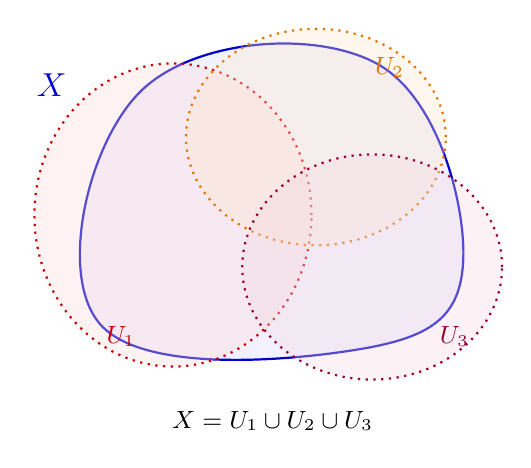
\begin{tikzpicture}[scale=1.1]
  \draw[blue!80!black, thick, fill=blue!5] plot[smooth cycle, tension=0.7] coordinates {(-2, -1.2) (-1.5, 1.5) (1.2, 1.8) (2.2, -0.5) (1.0, -1.5)};
  \node[blue!80!black, font=\large] at (-2.55, 1.55) {$X$};

  % The three sets must genuinely cover X -- ellipses chosen so every point of the
  % blob lies inside at least one of them (that is the whole point of a cover).
  \draw[red!80!black, thick, dotted, fill=red!15, fill opacity=0.35] (-1.15,0.05) ellipse (1.6 and 1.75);
  \node[red!80!black, font=\small] at (-1.75, -1.35) {$U_1$};

  \draw[orange!90!black, thick, dotted, fill=orange!20, fill opacity=0.35] (0.5,0.95) ellipse (1.5 and 1.25);
  \node[orange!90!black, font=\small] at (1.35, 1.75) {$U_2$};

  \draw[purple!80!black, thick, dotted, fill=purple!15, fill opacity=0.35] (1.15,-0.55) ellipse (1.5 and 1.3);
  \node[purple!80!black, font=\small] at (2.1, -1.35) {$U_3$};

  \node[below, font=\small] at (0, -2.1) {$X = U_1 \cup U_2 \cup U_3$};
\end{tikzpicture}
\end{center}

% Sonnet 5 (Medium)
